\documentclass[a4paper, 11pt]{article}
\usepackage[utf8]{inputenc}
\usepackage[left=1in,right=1in,bottom=0.8in]{geometry}
\usepackage{enumitem}
\usepackage{graphicx}
\graphicspath{ {Figures/} }
\usepackage{float}
\usepackage[labelfont=bf]{caption}
\usepackage{fixltx2e}
\usepackage{caption}
\usepackage{amsmath}
\usepackage{capt-of}
\usepackage{minted}
\usepackage{tabu}
\usepackage{pgf}
\usepackage{tikz}
\usetikzlibrary{arrows,automata}

\let\svthefootnote\thefootnote


\title{\bf Mid-Semester Examination\\\vspace*{2mm} BitCounter using the Krypton CPLD}
\author{\it Dhruv Ilesh Shah | 150070016}
\date{March 18, 2017}

\begin{document}
\maketitle
\section*{Overview}
In this experiment, we were expected to design a combinational circuit which calculates the number of input bits that are high, in a 16-bit input.

The code was compiled on Quartus Prime, and simulated using ModelSim. GHDL was also used for simulation purposes, at a low level. This was then uploaded to the {\em Krypton v1.1} 5M1270ZT144C5 CPLD-based board.

The algorithm and setup has been covered in section 1. We implement the counter in a parallel fashion, significantly reducing gate delays. The VHDL codes have been kept modular and as generic as possible, for reusability and code clarity. Section 2 presents the simulation observations and miscellaneous results. Section 3 presents the observations after running the scan-chain test on the board.

\section{Setup \& Algorithm}
The task is pretty trivial, and using a serial adder to add the 16 bits, although straight-forward, can cause a large amount of delay in the computation. It is also inefficient, as are adding the bits \emph{one at a time}. Instead, I used the following version of \emph{Divide \& Conquer}, specific to this case.

\begin{itemize}
	\item Group the bits into four groups, of four bits each.
	\begin{itemize}
		\item \texttt{b15 ... b12} $\rightarrow$ \texttt{int0}
		\item \texttt{b11 ... b8} $\rightarrow$ \texttt{int0}
		\item \texttt{b7 ... b4} $\rightarrow$ \texttt{int0}
		\item \texttt{b3 ... b0} $\rightarrow$ \texttt{int0}
	\end{itemize}
	\item Add the four bits in each group \emph{individually} using the entity \texttt{four\_bit\_linear} which generates a 4-bit output. This takes time equivalent to 4 serial additions instead of 16. The factor of 4 is compensated in memory.
	\item Take these 4 groups of 4-bit sums, and pool them together using a \texttt{FourBitAdder} which is basically a full adder.
\end{itemize}

The advantage of the above algorithm is that it causes significantly lower gate delays, as 4 computations are now occurring in a parallel setup.

\section{Observations}
Here, I present the results of running RTL \& Gate-Level Simulation on the design.
\subsection{RTL Simulation}
\begin{figure}[H]
\centering
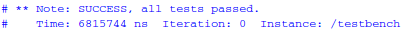
\includegraphics[scale=1]{RTL_Success}
\caption{RTL Simulation Result for the BitCounter}
\end{figure}

\begin{figure}[H]
\centering
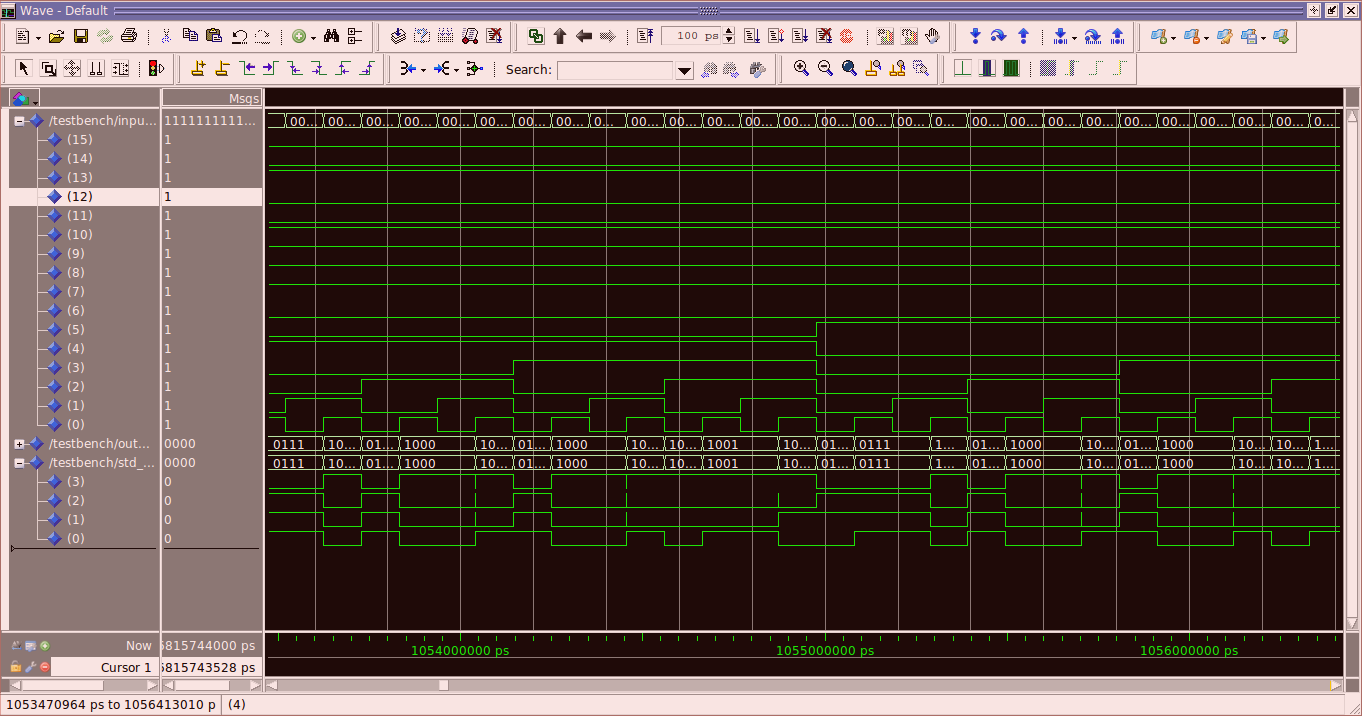
\includegraphics[scale=0.33]{RTL}
\caption{A snapshot RTL Simulation waveform on the BitCounter}
\end{figure}


\subsection{Gate-Level Simulation}
\begin{figure}[H]
\centering
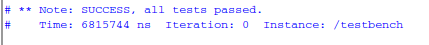
\includegraphics[scale=1]{Gate_Success}
\caption{Gate-Level Simulation Result for the BitCounter}
\end{figure}

\begin{figure}[H]
\centering
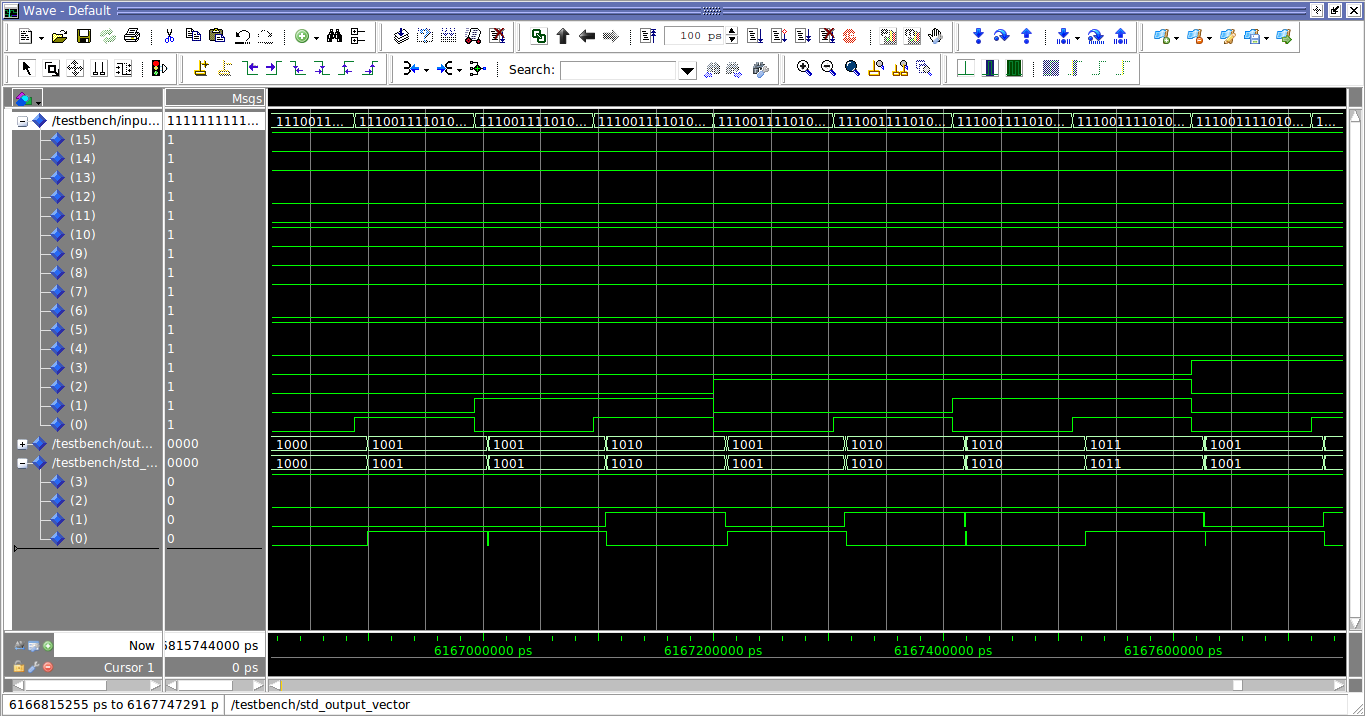
\includegraphics[scale=0.33]{Gate}
\caption{A snapshot gate-Level Simulation waveform on the BitCounter}
\end{figure}


\section{Scan-Chain Tests}
\begin{figure}[H]
\centering
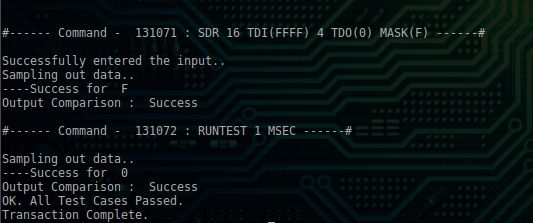
\includegraphics[scale=0.7]{Scan_Chain}
\caption{Result of running an exhaustive Scan Chain test on the board.}
\end{figure}

For the sake of completeness, Figure 6 shows output screens after running the Gate-Level (left) and Scan-Chain (right) tests.

\begin{figure}[H]
\centering
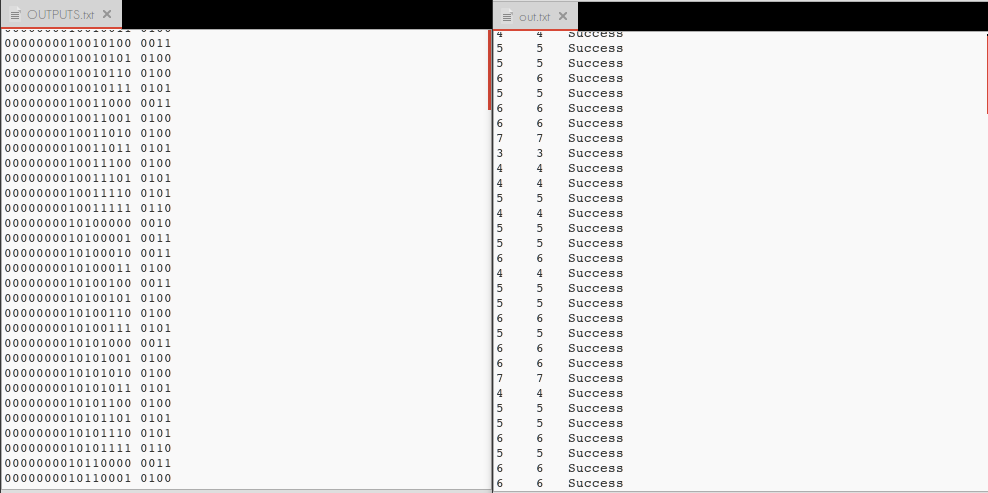
\includegraphics[scale=0.45]{Outputs}
\caption{Output screens after running the Gate-Level (left) and Scan-Chain (right) test.}
\end{figure}


\section*{Conclusion}
Starting from the very scratch, in this report, I have presented the logic and code for a combinational implementation of a bit counter. The logic was tested using RTL simulation, followed by the gate-level simulation for delay analysis and emulating the CPLD. This was followed by an actual rigorous test on the CPLD board after burning the code on it, using the \emph{TIVA-C} microcontroller.
\par
All the cases passed successfully at all stages and hence the complete bit counter can be used in hardware, as required.
\end{document}
